\documentclass{article}


% ready for submission
\usepackage{neurips_2022}


% to compile a preprint version, e.g., for submission to arXiv, add add the
% [preprint] option:
%     \usepackage[preprint]{neurips_2022}


% to compile a camera-ready version, add the [final] option, e.g.:
%     \usepackage[final]{neurips_2022}


% to avoid loading the natbib package, add option nonatbib:
%    \usepackage[nonatbib]{neurips_2022}


\usepackage[utf8]{inputenc} % allow utf-8 input
\usepackage[T1]{fontenc}    % use 8-bit T1 fonts
\usepackage{hyperref}       % hyperlinks
\usepackage{url}            % simple URL typesetting
\usepackage{booktabs}       % professional-quality tables
\usepackage{amsfonts}       % blackboard math symbols
\usepackage{nicefrac}       % compact symbols for 1/2, etc.
\usepackage{microtype}      % microtypography
\usepackage{xcolor}         % colors
\usepackage{graphicx}


\title{Reinforcement Learning for Portfolio Optimization Project Overview}

\begin{document}

\maketitle


\begin{abstract}
  The abstract paragraph should be indented \nicefrac{1}{2}~inch (3~picas) on
  both the left- and right-hand margins. Use 10~point type, with a vertical
  spacing (leading) of 11~points.  The word \textbf{Abstract} must be centered,
  bold, and in point size 12. Two line spaces precede the abstract. The abstract
  must be limited to one paragraph.
\end{abstract}


\section{Introduction}


Our group is seeking to develop a reinforcement learning agent to support portfolio 
management and optimization. Utilizing both empirical stock pricing data along with 
alternative data, we look to create a more well-informed portfolio optimization tool. 

Our primary motivations for pursuing a reinforcement learning-based approach are as 
follows:

\begin{enumerate}
    \item Reinforcement learning lends itself well to learning/opening in an online environment. The agent can interact with its environment, providing real-time feedback/ responsiveness to allow for better results.
    \item Our approach involves incorporating alternative data to support the agent’s decision making process. Encoding this alt-data into the states matrix of the agent allows for the agent to make better decisions when it comes to adjusting portfolio weights.
    \item Given that a reinforcement learning agent’s decisions are modeled by a Markov Decision Process, we can easily provide different reward functions to account for a variety of investor preferences or restrictions.
\end{enumerate}



A potential advisor for our project is Yada Zhu, a member of the finance research team 
at IBM. She was an author on one of the key papers we are referencing for our RL model 
implementation. Her experience with finance-related machine learning, time-series 
analysis, and alternative data sources would be very valuable in guiding us throughout 
our process.

Within our team, Sashwat and Ravi are working on dataset scraping, creation, curation, 
and cleaning; each is testing different APIs (described in the following section). 
Sumit and James are working on the RL algorithms; they are taking turns implementing 
papers described in that section and iterating on the architectures.




\section{Dataset Creation}

Creating a combined dataset encompassing a textual corpus sufficient for us to build 
a robust reinforcement learning agent will require pulling data from a wide variety 
of sources. We aim to use two primary types of data: stock and news data.

\subsection{Stock Data}

For now, since our project will likely be focused on building an agent that can perform 
well on historical data, we aim to use data from the Wharton Research Data Services 
(WRDS). WRDS is a pre-eminent source of financial data that we have experience 
utilizing in the Computational Finance program’s other courses that has expansive 
data on stocks. Specifically, we aim to use data from the Center for Research in 
Security Prices (CRSP), which has security price, return, and volume data for the 
NYSE, AMEX and NASDAQ stock markets. 

We will begin by creating a universe with just the S$\&$P 100 stocks, but we aim to 
expand to the S$\&$P 500 and/or stocks on all publicly-listed exchanges available through WRDS.

\subsection{News Data}

We believe that the inclusion of news data into our reinforcement learning agent’s 
state is important because it could integrate an external understanding of how 
well a given stock is performing at a given time and how it is specifically 
exposed to certain market or sector risks. This could provide our agent a better 
view of the environment and knowledge of our ticker companies in context, which 
can help it make better decisions to maximize our chosen reward function. To that 
end, we have a few proposed sources for pulling such data as well as a brief insight 
into our current progress towards that goal.


\subsubsection{Scraping Financial News Sources}

We want to focus on a few sites more committed to broadly reporting about a wide 
variety of companies to limit information asymmetry amongst stocks in our universe. 
News sources like Morningstar, Benzinga, and YFinance all allow users to filter their 
news searches by ticker. This will not only make it easier to scrape data, but also 
ensure that we actually have data for all of the companies in our universe. We plan
to collect at least a few years of data on each ticker, but one year of historical 
news articles for each ticker is a good starting point. Note that it is not essential 
for every ticker to have a news article for every day in our methodology. 

In scraping this data, we will be mindful of news organizations’ terms of 
services and ensure we are scraping ethically. Since the content is publicly 
available on these sites we will scrape at a reasonable frequency to avoid getting 
rate limited and/or IP blocked.

\subsubsection{Utilizing Paid News APIs}

Seeing a gap in real-time and historical data pipelines for business and professional 
use, many companies have created paid news APIs that allow institutions to query a 
wide range of news sites for current event information including financial news. 
Many of these APIs such as Event Registry, newsapi.ai, and Alpha Vantage provide 
this data. However, in examining most of these APIs there are a few significant 
issues. First, many of them require a significant payment to get data at a velocity 
that we would need. And for many, historical data is even more expensive. 

However, within the free tier of these services we can make some API calls to 
query information for some tickers that could be additive to our analysis. It would
be difficult to rely on this as a long term solution for data though.

\subsubsection{SEC Filings}

To enrich our dataset, we are considering utilizing SEC filings data for all 
NYSE/NASDAQ companies (available through WRDS) that we plan to pull data for. 
These filings contain essential information regarding a company's financial 
performance, governance, and compliance that could enhance our measure of 
company outlook. Specifically we aim to use data from 10-K and 10-Q filings. 
10-K’s are an annual report on a company’s performance, and include information. 
They are divided into items that show a company’s financial statements, 
stock projections, and pertinent information for shareholders in sections that 
are denoted as items. For our project, the textual data that is most likely to 
capture a company’s sentiment is Item 1A, Risk Factors. This item is a company 
issued statement on the risk factors that could affect the operations of the 
business for the next fiscal year. We will extract this data from 10-K statements 
for every company in our trading universe to create sentiment indicators for our 
RL agent to use. 

\subsection{Sentiment Analysis}

Using the news sources and SEC filings data described above, we wish to 
generate embeddings from which we can extract sentiment related features 
to provide to our reinforcement learning agent. Our initial approach, which 
we have conducted some basic testing on, is to utilize the pre-trained 
FinBERT model, fine-tuned to recognize the sentiment of financial text to 
create embeddings for us. 

\subsubsection{FinBERT Sentiment Scores}

For each time period, we will query headlines from articles about the individual 
stocks. Note that if we use a source like Benzinga, articles are already tagged 
with relevant stock tickers. We will feed headline data to pre-trained FinBERT. 
The model then will preprocess the text and generate probabilities of the content 
being positive, negative, or neutral. From there, we can assign each headline a 
numerical score based on its maximum probability class. The numerical map could 
look something like the following:  {positive: 1, neutral: 0, negative: -1} 
Over a trading period, we can take some aggregate of these class labels for 
each stock and feed these class labels to our agent’s states matrix; at each 
time step, this value will be appended to the row corresponding to the stocks’ 
price data. (The state matrix will be defined in greater detail in the Algorithmic 
and Analytical Challenges section.) We will experiment to find an optimal 
aggregate function; potential options include providing all logits, 
taking the mean, or designing a custom function to extract value heuristically. 
One such function could be
\[\texttt{Value}_{\texttt{Embedding}} = \tanh\Biggl( \frac{\frac{\texttt{positive sentiment probability}}{\texttt{negative sentiment probability}}}{\texttt{neutral sentiment probability}} \Biggr)\]
This approach combines the “log likelihood” (ratio of probabilities of positive and 
negative sentiment) along with a penalty for high neutral sentiment (a measure of 
uncertainty), using the tanh for normalization. This approach would allow us to 
adequately detect strong positive/negative sentiment. We will compare this against 
other aggregate functions in training experiments.

We will test the exact same preprocessing pipeline on the SEC 10-K and 10-Q filings 
for each company in our universe and integrate them into our states matrix. We will 
experiment with the same options mentioned previously for the optimal aggregation 
function. An issue that incorporates SEC filings is that they are recorded on a 
relatively infrequent basis compared to news and price data. Preliminarily, we will 
assume that there is no decay in the sentiment between reports. That means, 
the sentiment embeddings for each company will only be updated on dates where a
new filing was reported. On non-reporting dates, the embeddings will be filled 
forward from the last filing date. 

\subsubsection{Topic Modeling}

In a similar manner to the Financial Statement Analysis assignment from 
Andy Chakraborty’s lecture, we can also utilize FinBERT to categorize news 
headlines and content into financial-related topics. As demonstrated in that 
assignment, the correlations between such scores and the performance of 
companies can be useful to our RL agent by similarly incorporating such 
embeddings as a tensor. For every news headline and SEC filing related to 
each stock ticker, we will use the same pre-trained topic classification model 
as we did in our assignment to give us a numeric mapping of each text’s most 
probable topic. Using this, we will append a column of topic embeddings for 
each ticker on each day to the states matrix.

\section{Algorithmic and Analytical Challenge}

Our primary model technique is deep reinforcement learning, which is a 
branch of machine learning that operates in a game-theoretic-like system. 
Formally, a reinforcement learning problem is an instance of a Markov 
Decision Process, which is a 4-tuple (S, A, T, R): S the state space 
(matrix of selected historical stock price and news data available to 
our model at a given time; see Methodology section), A the action space 
(portfolio weights produced by our model, under appropriate constraints), 
T the transition function (how the state changes over time, modeled by our dataset), 
and R (the reward function). The goal is to find a policy (function from S to A) 
that maximizes future expected rewards. Most reinforcement learning research is 
spent on providing good information in S to the model, defining a good reward 
function R, and deciding on a deep learning model training system to optimize rewards.

\subsection{Existing Literature}

Much of the literature applying RL to portfolio optimization has arisen in the 
last few years. Some relevant papers are:

\begin{itemize}

\item $[2]$ Deep Reinforcement Learning for Optimal Portfolio Allocation: 
Using a lookback of recent past returns and a few market indicators 
(including 20-day volatility and the VIX), this paper implements a simple 
algorithm for portfolio weight selection to maximize the Differential Sharpe Ratio, 
a (local stepwise) reward function which approximates (global) Sharpe Ratio of the 
final strategy. They compare their model with the standard mean-variance 
optimization across several metrics.

\item $[3]$ DRL for Stock Portfolio Optimization Connected with Modern 
Portfolio Theory: This paper applies reinforcement learning methods to 
tensors of technical indicators and covariance matrices between stocks. 
After tensor feature extraction using 3D convolutions and tensor decompositions, 
the DDPG method is used to train the neural network policy, and the algorithm 
is backtested and compared against related methods.
 
\item $[6]$ RL-Based Portfolio Management with Augmented Asset Movement Prediction 
States: The authors propose a method to augment the state space S of historical 
price data with embeddings of internal information and alternative data. 
For all assets at all times, the authors use an LSTM to predict the price movement,
which is integrated into S. When news article data is available, different NLP methods 
are used to embed the news; this embedding is fed into an HAN to predict price 
movement, which is also integrated into S for state augmentation. The paper applies 
the DPG policy training method and compares against multiple baseline portfolios on 
multiple asset classes. It also addresses challenges due to environment uncertainty, 
sparsity, and news correlations.

\item $[1]$ A Deep Reinforcement Learning Framework for the Financial Portfolio Management Problem: 
This paper contains a deep mathematical and algorithmic discussion of how to properly incorporate 
transaction costs into an RL model. The authors also have a GitHub with implementations of their 
RL strategy compared with several others.

\item $[7]$ Stock Portfolio Selection Using Learning-to-Rank Algorithms with News Sentiment: 
After developing news sentiment indicators including shock and trends, this paper applies 
multiple learning-to-rank algorithms and constructs an automated trading system with strong performance.

\item $[5]$ MAPS: Multi-agent Reinforcement Learning-based Portfolio Management System: 
This paper takes advantage of reinforcement learning with multiple agents by defining a 
reward function to penalize correlations between agents, thereby producing multiple orthogonal 
(diverse) high-performing portfolios.

\end{itemize}

\subsection{Methodology}

We will be implementing, combining, and improving on the methodologies of several of the above papers. 
Our plan is to develop an RL system that utilizes multiple time periods to achieve strong out-of-sample 
trading performance. As of this writing, we have partial implementations of papers $[1]$, $[2]$, and $[3]$.
 Our final architecture will be most similar to papers $[6]$ and $[1]$.

\subsubsection{Markov Decision Process Problem Formulation}

Paper $[6]$ includes the following diagram, which is very close to our desired 
architecture:

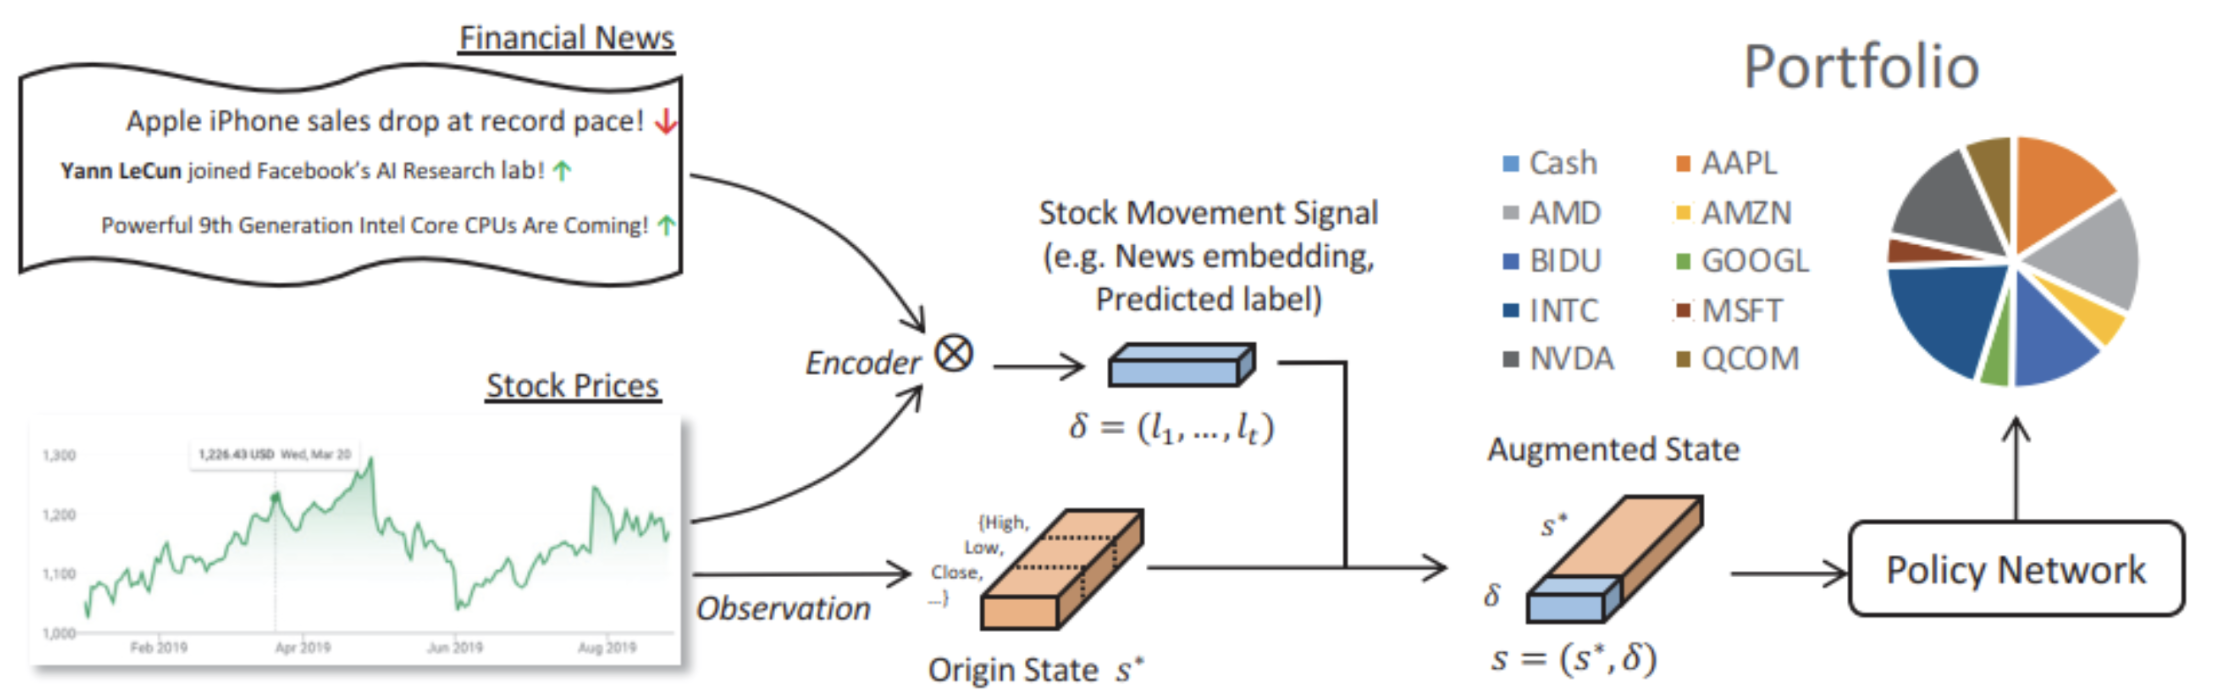
\includegraphics[width=13cm]{formulation.png}

An explanation of this diagram: at time t, the origin state S* is a 3D tensor of dimensions $U \times H \times C$
which contains historical price data. U is the size of our universe (for example, for the S$\&$P100, U=100). 
H is the size of history we are providing (if we are providing 30 day history, then H = 30). 
C is a categorical value representing the close/high/low price. This format of S* allows us to store, 
for example, the last 30 days of stock price data for all companies in the S$\&$P100, for any given day. 
In addition to this, we have news information Delta, obtained from financial news headlines for that day, 
processed through a pre-trained encoder. This information is added to S* to create the full state 
S = (S*, Delta)

In our architecture, for S*, we will experiment with the lookback period size and likely reduce it 
to a 2D array by flattening along the C index, but will otherwise keep S* largely the same. For 
Delta, we plan to utilize better feature extraction via sentiment scores and topic modeling; 
we also plan to use different alternative data sources, as described in the Dataset Creation section. 
In addition, we will extract what company each headline refers to, so our features can be changed 
over time independently for each company as news articles enter through our environment. The final 
state S will likely be a 2D matrix, where each row represents a different company (ticker), and along 
that row we find, concatenated, the following: (1) the past month-or-so of stock price data from S*, 
and (2) numerical features extracted from recent news data pertinent to that company (as described 
in the Dataset section). (The straightforward concatenation of price data and news embeddings did not 
affect the ability of the neural network-based agent to learn.)

Regarding the reward function R, we plan to experiment with both the profit reward function used in $[6]$, 
as well as the Differential Sharpe Ratio developed in paper $[2]$.

In summary, our project aims to implement and replicate the approach used in $[6]$, with 
some modifications to S and R as previously described. We will conduct experiments alternative data 
sources, feature extraction methods, and reward functions (both custom and from other papers listed) 
to find a good combination that allows this approach to work well on S$\&$P100 stocks; this comprises our 
novel extension/contribution.

\subsubsection{Use of Libraries}

We will mainly be using the Gymnasium library to implement the reinforcement learning environments. 
The Stable Baselines 3 library provides several policy learning techniques that we will experiment with, 
including Proximal Policy Optimization (PPO) and Deep Deterministic Policy Gradients (DDPG). 
The papers above discuss the advantages and disadvantages of multiple reward functions and constraints, 
which we will make improvements upon and provide as options to the user, if applicable.

\subsubsection{Strategy Benchmarking}

Our final model architecture will be compared against several benchmark financial portfolio selection 
models. Among these will be the CAPM, an exponential moving average strategy, linear factor models 
such as the Fama French 3/5-factor models, and the QMJ model. We will compare our returns 
in-sample and out-of-sample plots, as well as our relative performance on portfolio statistics 
including cumulative return, Sharpe Ratio, Sortino Ratio, drawdown, etc. The experiment sections 
in the above papers provide a strong reference for our methodological comparison.

\section{User Interface and Visual Analytics}

As our project is primarily oriented towards data curation and algorithms, we will not directly have a 
user interface for a final end-user. However, in order to experiment with and visualize the performance 
of our various models, we will create a small suite of visualizations in an interactive manner that 
allows a researcher to choose methods and hyperparameters for our architecture. We will also create a 
notebook to demonstrate the infrastructure and usage of our deep reinforcement learning model, 
similar to those on TensorFlow and Huggingface.

\section{References}

$[1]$ Z. Jiang, D. Xu, and J. Liang, “A Deep Reinforcement Learning Framework for the Financial Portfolio Management Problem.” arXiv, Jul. 16, 2017. Accessed: Mar. 29, 2024. [Online]. Available: http://arxiv.org/abs/1706.10059

$[2]$ S. Sood, K. Papasotiriou, M. Vaiciulis, and T. Balch, “Deep Reinforcement Learning for Optimal Portfolio Allocation: A Comparative Study with Mean-Variance Optimization”.

$[3]$ J. Jang and N. Seong, “Deep reinforcement learning for stock portfolio optimization by connecting with modern portfolio theory,” Expert Systems with Applications, vol. 218, p. 119556, May 2023, doi: 10.1016/j.eswa.2023.119556.

$[4]$ S. Gössi, Z. Chen, W. Kim, B. Bermeitinger, and S. Handschuh, “FinBERT-FOMC: Fine-Tuned FinBERT Model with Sentiment Focus Method for Enhancing Sentiment Analysis of FOMC Minutes,” in Proceedings of the Fourth ACM International Conference on AI in Finance, in ICAIF ’23. New York, NY, USA: Association for Computing Machinery, Nov. 2023, pp. 357–364. doi: 10.1145/3604237.3626843.

$[5]$ J. Lee, R. Kim, S.-W. Yi, and J. Kang, “MAPS: Multi-agent Reinforcement Learning-based Portfolio Management System,” in Proceedings of the Twenty-Ninth International Joint Conference on Artificial Intelligence, Jul. 2020, pp. 4520–4526. doi: 10.24963/ijcai.2020/623.

$[6]$ Y. Ye et al., “Reinforcement-Learning based Portfolio Management with Augmented Asset Movement Prediction States.” arXiv, Feb. 09, 2020. doi: 10.48550/arXiv.2002.05780.

$[7]$ Q. Song, A. Liu, and S. Y. Yang, “Stock portfolio selection using learning-to-rank algorithms with news sentiment,” Neurocomputing, vol. 264, pp. 20–28, Nov. 2017, doi: 10.1016/j.neucom.2017.02.097.



% \section{Preparing PDF files}


% Please prepare submission files with paper size ``US Letter,'' and not, for
% example, ``A4.''


% Fonts were the main cause of problems in the past years. Your PDF file must only
% contain Type 1 or Embedded TrueType fonts. Here are a few instructions to
% achieve this.


% \begin{itemize}


% \item You should directly generate PDF files using \verb+pdflatex+.


% \item You can check which fonts a PDF files uses.  In Acrobat Reader, select the
%   menu Files$>$Document Properties$>$Fonts and select Show All Fonts. You can
%   also use the program \verb+pdffonts+ which comes with \verb+xpdf+ and is
%   available out-of-the-box on most Linux machines.


% \item The IEEE has recommendations for generating PDF files whose fonts are also
%   acceptable for NeurIPS. Please see
%   \url{http://www.emfield.org/icuwb2010/downloads/IEEE-PDF-SpecV32.pdf}


% \item \verb+xfig+ "patterned" shapes are implemented with bitmap fonts.  Use
%   "solid" shapes instead.


% \item The \verb+\bbold+ package almost always uses bitmap fonts.  You should use
%   the equivalent AMS Fonts:
% \begin{verbatim}
%    \usepackage{amsfonts}
% \end{verbatim}
% followed by, e.g., \verb+\mathbb{R}+, \verb+\mathbb{N}+, or \verb+\mathbb{C}+
% for $\mathbb{R}$, $\mathbb{N}$ or $\mathbb{C}$.  You can also use the following
% workaround for reals, natural and complex:
% \begin{verbatim}
%    \newcommand{\RR}{I\!\!R} %real numbers
%    \newcommand{\Nat}{I\!\!N} %natural numbers
%    \newcommand{\CC}{I\!\!\!\!C} %complex numbers
% \end{verbatim}
% Note that \verb+amsfonts+ is automatically loaded by the \verb+amssymb+ package.


% \end{itemize}


% If your file contains type 3 fonts or non embedded TrueType fonts, we will ask
% you to fix it.


% \subsection{Margins in \LaTeX{}}


% Most of the margin problems come from figures positioned by hand using
% \verb+\special+ or other commands. We suggest using the command
% \verb+\includegraphics+ from the \verb+graphicx+ package. Always specify the
% figure width as a multiple of the line width as in the example below:
% \begin{verbatim}
%    \usepackage[pdftex]{graphicx} ...
%    \includegraphics[width=0.8\linewidth]{myfile.pdf}
% \end{verbatim}
% See Section 4.4 in the graphics bundle documentation
% (\url{http://mirrors.ctan.org/macros/latex/required/graphics/grfguide.pdf})


% A number of width problems arise when \LaTeX{} cannot properly hyphenate a
% line. Please give LaTeX hyphenation hints using the \verb+\-+ command when
% necessary.


% \begin{ack}
% Use unnumbered first level headings for the acknowledgments. All acknowledgments
% go at the end of the paper before the list of references. Moreover, you are required to declare
% funding (financial activities supporting the submitted work) and competing interests (related financial activities outside the submitted work).
% More information about this disclosure can be found at: \url{https://neurips.cc/Conferences/2022/PaperInformation/FundingDisclosure}.


% Do {\bf not} include this section in the anonymized submission, only in the final paper. You can use the \texttt{ack} environment provided in the style file to autmoatically hide this section in the anonymized submission.
% \end{ack}


% \section*{References}


% References follow the acknowledgments. Use unnumbered first-level heading for
% the references. Any choice of citation style is acceptable as long as you are
% consistent. It is permissible to reduce the font size to \verb+small+ (9 point)
% when listing the references.
% Note that the Reference section does not count towards the page limit.
% \medskip


% {
% \small


% [1] Alexander, J.A.\ \& Mozer, M.C.\ (1995) Template-based algorithms for
% connectionist rule extraction. In G.\ Tesauro, D.S.\ Touretzky and T.K.\ Leen
% (eds.), {\it Advances in Neural Information Processing Systems 7},
% pp.\ 609--616. Cambridge, MA: MIT Press.


% [2] Bower, J.M.\ \& Beeman, D.\ (1995) {\it The Book of GENESIS: Exploring
%   Realistic Neural Models with the GEneral NEural SImulation System.}  New York:
% TELOS/Springer--Verlag.


% [3] Hasselmo, M.E., Schnell, E.\ \& Barkai, E.\ (1995) Dynamics of learning and
% recall at excitatory recurrent synapses and cholinergic modulation in rat
% hippocampal region CA3. {\it Journal of Neuroscience} {\bf 15}(7):5249-5262.
% }


% %%%%%%%%%%%%%%%%%%%%%%%%%%%%%%%%%%%%%%%%%%%%%%%%%%%%%%%%%%%%
% \section*{Checklist}


% %%% BEGIN INSTRUCTIONS %%%
% The checklist follows the references.  Please
% read the checklist guidelines carefully for information on how to answer these
% questions.  For each question, change the default \answerTODO{} to \answerYes{},
% \answerNo{}, or \answerNA{}.  You are strongly encouraged to include a {\bf
% justification to your answer}, either by referencing the appropriate section of
% your paper or providing a brief inline description.  For example:
% \begin{itemize}
%   \item Did you include the license to the code and datasets? \answerYes{See Section~\ref{gen_inst}.}
%   \item Did you include the license to the code and datasets? \answerNo{The code and the data are proprietary.}
%   \item Did you include the license to the code and datasets? \answerNA{}
% \end{itemize}
% Please do not modify the questions and only use the provided macros for your
% answers.  Note that the Checklist section does not count towards the page
% limit.  In your paper, please delete this instructions block and only keep the
% Checklist section heading above along with the questions/answers below.
% %%% END INSTRUCTIONS %%%


% \begin{enumerate}


% \item For all authors...
% \begin{enumerate}
%   \item Do the main claims made in the abstract and introduction accurately reflect the paper's contributions and scope?
%     \answerTODO{}
%   \item Did you describe the limitations of your work?
%     \answerTODO{}
%   \item Did you discuss any potential negative societal impacts of your work?
%     \answerTODO{}
%   \item Have you read the ethics review guidelines and ensured that your paper conforms to them?
%     \answerTODO{}
% \end{enumerate}


% \item If you are including theoretical results...
% \begin{enumerate}
%   \item Did you state the full set of assumptions of all theoretical results?
%     \answerTODO{}
%         \item Did you include complete proofs of all theoretical results?
%     \answerTODO{}
% \end{enumerate}


% \item If you ran experiments...
% \begin{enumerate}
%   \item Did you include the code, data, and instructions needed to reproduce the main experimental results (either in the supplemental material or as a URL)?
%     \answerTODO{}
%   \item Did you specify all the training details (e.g., data splits, hyperparameters, how they were chosen)?
%     \answerTODO{}
%         \item Did you report error bars (e.g., with respect to the random seed after running experiments multiple times)?
%     \answerTODO{}
%         \item Did you include the total amount of compute and the type of resources used (e.g., type of GPUs, internal cluster, or cloud provider)?
%     \answerTODO{}
% \end{enumerate}


% \item If you are using existing assets (e.g., code, data, models) or curating/releasing new assets...
% \begin{enumerate}
%   \item If your work uses existing assets, did you cite the creators?
%     \answerTODO{}
%   \item Did you mention the license of the assets?
%     \answerTODO{}
%   \item Did you include any new assets either in the supplemental material or as a URL?
%     \answerTODO{}
%   \item Did you discuss whether and how consent was obtained from people whose data you're using/curating?
%     \answerTODO{}
%   \item Did you discuss whether the data you are using/curating contains personally identifiable information or offensive content?
%     \answerTODO{}
% \end{enumerate}


% \item If you used crowdsourcing or conducted research with human subjects...
% \begin{enumerate}
%   \item Did you include the full text of instructions given to participants and screenshots, if applicable?
%     \answerTODO{}
%   \item Did you describe any potential participant risks, with links to Institutional Review Board (IRB) approvals, if applicable?
%     \answerTODO{}
%   \item Did you include the estimated hourly wage paid to participants and the total amount spent on participant compensation?
%     \answerTODO{}
% \end{enumerate}


% \end{enumerate}


%%%%%%%%%%%%%%%%%%%%%%%%%%%%%%%%%%%%%%%%%%%%%%%%%%%%%%%%%%%%


% \appendix


% \section{Appendix}


% Optionally include extra information (complete proofs, additional experiments and plots) in the appendix.
% This section will often be part of the supplemental material.


\end{document}